\section{Experiments}
\subsection{Stress-buffering Effect of Positive Events}
\label{subsec:experiment}
In short,
we explored the stress-buffering effect of specific positive events based on the framework from section \ref{sec:frame}.
Four positive scheduled events were adopted:
practical activities, holidays, New Year parties and sporting events.
Table \ref{tab:schedule} shows the experimental results,
where 54.52\%, 78.39\%, 63.39\%, 58.74\% significant stress-buffering effects were detected for
each of the four positive scheduled events, respectively,
with a total ratio of 69.52\% ($\alpha$ =1.96 for P=0.025).
Here, the Pearson correlation coefficient was calculated to compare with the statistical model in section \ref{sec:frame2}.
The Euclidean distance was used to calculate the distance between two $n$-dimensional points $X$ and $Y$.
The experimental results showed that our KNN-based two-sample method (called KTS)
outperformed the baseline method with the best improvement in event \emph{New Year parties} to 10.94\%,
and the total improvement by 6.00\%.

\begin{table}
\begin{center}
\caption{\small{Quantification of the stress-buffering effect of positive scheduled events applying
the KTS model (the KNN-based two-sample method adopted in this research) and the baseline method.}}
\label{tab:schedule}
\resizebox{0.45\textwidth}{13mm}{
\small{
\begin{tabular}{lccccc}
\toprule
&	Practical	&	         	&	New Year	&	Sporting	&	\\
&	activity	&	Holiday	&	party	&	events	&	All	\\
\midrule
Size of U-SI	&	219 	&	339 	&	235 	&	226 	&	1,019 	\\
Pearson         &55.65\%	&	70.97\%	&	56.45\%	&	54.84\%	&	65.32\% \\
KTS             &54.52\%	&	78.39\%	&	63.39\%	&	58.74\%	&	69.52\% \\
\bottomrule
\end{tabular}
}
}
\end{center}
\end{table}

The stress-buffering effects measured by three groups of microblogging characteristics
and towards the five dimensions of stressor events are shown in box plots \ref{fig:correlation},
using the statistical $\alpha$ value computed via the KTS method.
The results showed the stress-buffering pattern of positive events
was significantly correlated with posting behaviors (ratio = 83.06\%, n=103, SD=1.96),
stress-change modes (ratio = 74.19\%, n=92, SD=2.04) and linguistic expressions (ratio = 77.42\%, n=96, SD=2.07).
Positive events had the most significant stress-buffering impact on 'family life' (ratio = 84.68\%, n=105, SD=2.72),
followed by 'peer relationships' (ratio = 79.03\%, n=98, SD=4.04) and 'school life' (ratio = 68.55\%, n=85, SD=2.71).
The $\alpha$ for 'peer relationships' exhibited the highest 75th percentile and the lowest 25th percentile,
showing a relatively random and unstable stress-buffering effect on this dimension.
Comparing the hypothesis test results on the positive scheduled events (ratio = 69.52\%)
and automatically extracted positive events (ratio = 74.21\%),
the results indicated the feasibility of automatically extracting positive events from microblogs.

\begin{figure}
\centering
\includegraphics[width=\linewidth]{figs/cor.eps}%figs/correlation2.eps
\caption{\small{ Subgraph (a) shows the statistical $\alpha$ value of each group of measures.
Subgraph (b) shows the stress-buffering effects on five dimensions of stressors.}}
\label{fig:correlation}
\end{figure}

Next,
to verify monotonic changes in stress intensity when a positive event impacted a stressful interval,
for each interval in the SI and U-SI sets,
we quantified its monotonous stress changes by comparing it with the front- and rear-adjacent intervals, respectively.
Four situations proposed in section \ref{sec:mono} were considered and are compared in Table \ref{tab:fontrear}.
The ratio of intervals detected with the monotonic increase from the front interval to the current stressful interval $I$
(denoted by \emph{front$ \rightarrow$ I}),
and the ratio of the monotonic decrease from $I$ to its rear-adjacent interval (denoted by \emph{I $\rightarrow$ rear}) are summarized.
Under the effect of positive events,
the ratio of intensive stress increase in \emph{front$ \rightarrow$ I} was reduced from 78.51\% to 70.17\%;
the ratio of intensive stress decrease in \emph{I $\rightarrow$ rear} was reduced from 79.55\% to 75.13\%.
The most obvious monotonic decrease in \emph{front$ \rightarrow$ I} was related to positive events
in the 'family life' dimension (12.89\% reduction),
and the most obvious monotonic decrease in \emph{front$ \rightarrow$ I} was also related to positive events in the 'family life' dimension (6.65\% reduction).
The experimental results indicate the effectiveness of the two-sample methods for quantifying the effect of positive events
and the rationality of the assumption that positive events could help ease the stress of overwhelmed adolescents.


\begin{table*}
\caption{\small{Adolescents' stress prediction performance when combining different groups of stress-buffering measures separately.}}
\begin{minipage}{\linewidth}
\centering
\resizebox{\textwidth}{20mm}{
\begin{tabular}{l cccc cccc cccc cccc} \\\hline%\toprule
\multirow{2}{1cm}{}&\multicolumn{4}{c}{None}
    &\multicolumn{4}{c }{Positive (L)}
    &\multicolumn{4}{c }{Positive (S)}
    &\multicolumn{4}{c}{Positive (P)}\\
    &\scriptsize{MSE} &\scriptsize{RMSE} &\scriptsize{MAPE} &\scriptsize{MAD}
    &\scriptsize{MSE} &\scriptsize{RMSE} &\scriptsize{MAPE} &\scriptsize{MAD}
    &\scriptsize{MSE} &\scriptsize{RMSE} &\scriptsize{MAPE} &\scriptsize{MAD}
    &\scriptsize{MSE} &\scriptsize{RMSE} &\scriptsize{MAPE} &\scriptsize{MAD} \\\midrule					
School life
&   0.0856 	&	0.2926 	&	0.4852 	&	0.1146	&	0.0259 	&	0.1609 	&	0.2991 	&	0.0923 	
&	0.0297 	&	0.1723 	&	0.3135 	&	0.0899 	&	0.0223 	&	0.1493 	&	0.3438 	&	0.0931 	\\
Romantic relationships
&   0.0703 	&	0.2651 	&	0.3555 	&	0.1083 	&	0.0291 	&	0.1706 	&	0.2832 	&	0.0919 	
&	0.0379 	&	0.1947 	&	0.2941 	&	0.1026 	&	0.0332 	&	0.0835 	&	0.2746 	&	0.1240 	\\
Peer relationships
&   0.2800 	&	0.5292 	&	0.3256 	&	0.1697 	&	0.3140 	&	0.5604 	&	0.3626 	&	0.1202 	
&	0.2972 	&	0.5452 	&	0.3060 	&	0.1298 	&	0.2557 	&	0.1472 	&	0.3481 	&	0.1458 	\\
Self-cognition
&   0.0445 	&	0.2110 	&	0.3066 	&	0.1895 	&	0.0345 	&	0.1857 	&	0.2721 	&	0.1653 	
&	0.0366 	&	0.1913 	&	0.2557 	&	0.0754 	&	0.0245 	&	0.0862 	&	0.2863 	&	0.1447 	\\
Family life
&   0.1602 	&	0.4002 	&	0.3291 	&	0.1587 	&	0.0889 	&	0.2982 	&	0.2891 	&	0.0944 	
&	0.0378 	&	0.1944 	&	0.2952 	&	0.0842 	&	0.1827 	&	0.0979 	&	0.3148 	&	0.1131 	\\
All	
&   0.1281 	&	0.3579 	&	0.3604 	&	0.1482	&	0.0985 	&	0.3138 	&	0.3012 	&	0.1128 	
&	0.0878 	&	0.2964 	&	0.2929 	&	0.0964 	&	0.1037 	&	0.1128 	&	0.3135 	&	0.1241 	\\ \hline
\end{tabular}}
\end{minipage}\\
\begin{minipage}{\linewidth}
\centering
\resizebox{\textwidth}{20mm}{
\begin{tabular}{l cccc cccc cccc cccc} \\\hline%\toprule
\multirow{2}{1cm}{}&\multicolumn{4}{c}{Positive (L\&S)}
    &\multicolumn{4}{c }{Positive (L\&P)}
    &\multicolumn{4}{c }{Positive (S\&P)}
    &\multicolumn{4}{c}{Positive (L\&S\&P)}\\
    &\scriptsize{MSE} &\scriptsize{RMSE} &\scriptsize{MAPE} &\scriptsize{MAD}
    &\scriptsize{MSE} &\scriptsize{RMSE} &\scriptsize{MAPE} &\scriptsize{MAD}
    &\scriptsize{MSE} &\scriptsize{RMSE} &\scriptsize{MAPE} &\scriptsize{MAD}
    &\scriptsize{MSE} &\scriptsize{RMSE} &\scriptsize{MAPE} &\scriptsize{MAD} \\\midrule					
School life
&	0.0283 	&	0.1682 	&	0.2934 	&	0.0824 	&	0.0261 	&	0.1616 	&	0.2770 	&	0.0768 	
&	0.0342 	&	0.1849 	&	0.2629 	&	0.0590 	&	0.0132 	&	0.1149 	&	0.2364 	&	0.0717 	\\
Romantic relationships
&	0.0219 	&	0.1480 	&	0.2532 	&	0.0839 	&	0.0180 	&	0.1342 	&	0.2644 	&	0.0952 	
&	0.0176 	&	0.1327 	&	0.2549 	&	0.0823 	&	0.0251 	&	0.1584 	&	0.2507 	&	0.0891 	\\
Peer relationships
&	0.2361 	&	0.4859 	&	0.3182 	&	0.1300 	&	0.2349 	&	0.4847 	&	0.3283 	&	0.1189 	
&	0.2351 	&	0.4849 	&	0.3558 	&	0.1297 	&	0.2341 	&	0.4838 	&	0.3096 	&	0.1093 	\\
Self-cognition
&	0.0329 	&	0.1814 	&	0.2942 	&	0.0946 	&	0.0262 	&	0.1619 	&	0.2791 	&	0.0858 	
&	0.0245 	&	0.1565 	&	0.2740 	&	0.0945 	&	0.0144 	&	0.1200 	&	0.2580 	&	0.0739 	\\
Family life
&	0.1489 	&	0.3859 	&	0.2750 	&	0.1244 	&	0.0395 	&	0.1987 	&	0.2853 	&	0.0939 	
&	0.0484 	&	0.2200 	&	0.2946 	&	0.0992 	&	0.0378 	&	0.1944 	&	0.2645 	&	0.0848 	\\
All
&	0.0936 	&	0.3060 	&	0.2868 	&	0.1031 	&	0.0689 	&	0.2626 	&	0.2868 	&	0.0941 	&	0.0720 	&	0.2683 	&	0.2884 	&	0.0929 	&	0.0649 	&	0.2548 	&	0.2638 	&	0.0858 	\\ \hline
\end{tabular}}
\begin{tablenotes}
        \footnotesize
        \item[1] $^1$ Three stress-buffering measures: 'L' represents \emph{linguistic expression}, 'S' represents \emph{stress intensity}, and 'P' represents \emph{posting behavior}.
      \end{tablenotes}
\end{minipage}
\label{tab:forecast}
\end{table*}

\subsection{Predicting Future Stress Under the Stress-buffering Effects of Positive Events}
\label{subsec:predict}
To further explore the effectiveness of our method for quantifying the stress-buffering effects of positive events,
we integrate the impact of positive events into a stress prediction problem
and verify whether considering the stress-buffering effects of positive events could help improve the stress prediction performance.


\paragraph{Stress prediction model}
The SVARIMA (seasonal autoregressive integrated moving average) algorithm was proven to be suitable for the adolescents' stress prediction problem \citep{Li2015Predicting, Shumway2006Time},
due to the seasonality and nonstationarity of the stress series.
Since stressor events cause the fluctuation in the stress series from normal states,
we focused the prediction problem on stressful intervals rather than randomly selected stress series.
Thus, basic stress prediction was conducted using the SVARIMA approach in the set of stressful intervals impacted by positive events (U-SI).
Stress-buffering effects of positive events were adopted as adjust values to modify the stress prediction results.
Four metrics were adopted to measure the stress-forecasting performance:
\emph{MSE}, \emph{RMSE} and \emph{MAD} measure the absolute errors,
and \emph{MAPE} measures the relative measures.
For all real stress values $\overline{s_i}$ and predicted stress values $s_i$ in a prediction sequence $<s_1,\cdots,s_n>$:
$MSE = \frac{1}{n}\sum_{i\in[1,n]}(s_i-\overline{s_i})^2$,
$RMSE = \frac{1}{n}\sqrt{\sum_{i\in[1,n]}(s_i-\overline{s_i})^2}$,
$MAD = \frac{1}{n}\sum_{i\in[1,n]}|s_i-\overline{s_i}|$,
$MAPE = $ $\frac{1}{n}$ $\sum_{i\in[1,n]}{|s_i-\overline{s_i}|/s_i}$.

The experimental set contained 1,914 stressful intervals under the impact of positive events (U-SI).
As shown in Table \ref{tab:forecast},
the original prediction performance using only the SVARIMA method
achieved an MSE of 0.1281, an RMSE of 0.3579, a MAPE of 0.3604 and a MAD of 0.1482 ($L = 7$, $\beta = 0.5$).
Then we integrated the stress-buffering impact of each dimension of positive events for stress prediction.
Specifically, for positive events leading to significant stress-buffering effects on the current adolescent,
the average stress value during historical U-SI intervals was integrated to modify the result by adjusting the parameter $\beta$.
After modification,
the prediction performance achieved an MSE of 0.0649, an RMSE of 0.2548, a MAPE of 0.2638 and a MAD of 0.0858,
reducing the prediction errors efficiently (the MSE, RMSE, MAPE and MAD were reduced by 49.34\%, 28.81\%, 26.80\% and 42.11\%, respectively).

\paragraph{Contribution of each group of measures}
Further,
we conducted experiments with different stress-buffering patterns included to show each pattern's contribution to stress prediction.
Four groups of situations were considered here, as shown in Table \ref{tab:forecast},
considering
1) all three groups of measures, namely, stress-change modes, linguistic expressions and posting behaviors (the L\&S\&P pattern),
2) any two of the three groups of measures included (the L$|$S, L\&P, and S\&P patterns),
3) only one group of measures included (the L, S, or P patterns),
and 4) none of the measures included.
We integrated the effect of positive events under the four situations for stress prediction
by the overlapping parameter $\alpha \times S_{historical}$,
where $S_{historical}$ is the average stress value in the historical U-SI intervals.
Here, we present the prediction result when $\beta = 0.5$ in each dimension of stress.
The results showed that the stress-buffering pattern in the L\&S\&P pattern outperformed the other patterns
(MSE = 0.0649, RMSE = 0.2548, MAPE = 0.2638 and MAD = 0.0858),
showing the effectiveness of all three groups of measures.
\begin{figure*}
\centering
\caption{\small{Adolescents' stress prediction performance under different observation window lengths.}}
\includegraphics[width=\linewidth]{figs/predictWindow2.eps}
\label{fig:length}
\end{figure*}

\paragraph{Stress prediction performance under different observation window lengths}
We further explored combing stress-buffering effects into future stress prediction under different lengths of observation windows,
ranging from 1 to 10 days, as shown in Figure \ref{fig:length}.
With increasing window length,
the prediction errors showed an increasing trend across all the metrics.
The reason might be that a longer prediction window resulted in more previously predicted results
and errors accumulating with more predicted values are taken into the next step of prediction.
Among the five dimensions of stressor events,
the prediction for school-life stress achieved the best performance.
One reason might be that more positive events and stressors about school-life events were detected from adolescents' microblogs,
providing sufficient data in the prediction process.
On the other hand,
stress coming from school life was the most common source of stress in the student group with relatively stable periodicity,
which was more suitable for the current prediction model.


\begin{figure}
\centering
\caption{\small{Stress prediction performance under the L\&S\&P stress-buffering pattern of positive events.}}
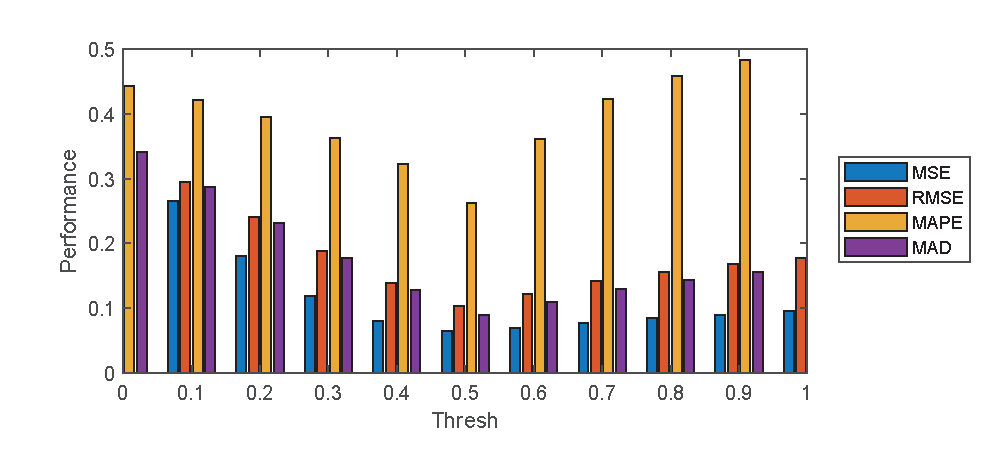
\includegraphics[width=\linewidth]{figs/thresh.eps}
\label{fig:thresh}
\end{figure}

\paragraph{Parameter settings}
$\beta$ was adjusted when the impact of positive events was integrated into stress prediction.
For each of the four groups of stress-buffering patterns,
we adjust $\beta$ to the effect of $\beta \times L$.
We calculated the corresponding prediction result for each adolescent as follows,
and showed the result of the entire testing group in the average performance.
Figure \ref{fig:thresh} shows the changing trend under the L\&S\&P pattern.
The prediction errors decreased first and then increased,
and the best performance was achieved when $\beta$ was
approximately 0.52, with an MSE of 0.0649, an RMSE of 0.2548,
a MAPE of 0.2638 and a MAD of 0.0858 as the average performance of the entire experimental dataset.
Multiple methods for integrating the stress-buffering impact of positive events into stress prediction could be adopted in the future.
In this paper,
we adopted a simple method to verify the effectiveness of our model in quantifying the impact of positive events.
The setting of $\beta$ could be changed according to different individuals and datasets.
